\section{Simulation Analysis}
\label{sec:simulation}

\subsection{Operating Point Analysis}

Table~\ref{tab:op} shows the simulated operating point results for the circuit
under analysis. Compared to the theoretical analysis results, one notices the
following differences: describe and explain the differences.

\begin{table}[h]
  \centering
  \begin{tabular}{|l|r|}
    \hline    
    {\bf Name} & {\bf Value [A or V]} \\ \hline
    @gb[i] & -2.47520e-04\\ \hline
@id[current] & 1.005321e-03\\ \hline
@r1[i] & 2.364560e-04\\ \hline
@r2[i] & -2.47520e-04\\ \hline
@r3[i] & -1.10640e-05\\ \hline
@r4[i] & 1.201119e-03\\ \hline
@r5[i] & -1.25284e-03\\ \hline
@r6[i] & 9.646630e-04\\ \hline
@r7[i] & 9.646630e-04\\ \hline
v(1) & 5.076387e+00\\ \hline
v(2) & 4.828240e+00\\ \hline
v(3) & 4.317615e+00\\ \hline
v(4) & 4.862301e+00\\ \hline
v(5) & 8.665725e+00\\ \hline
v(6) & -1.94693e+00\\ \hline
v(7) & -2.95363e+00\\ \hline
v(9) & -1.94693e+00\\ \hline

  \end{tabular}
  \caption{Operating point. A variable preceded by @ is of type {\em current}
    and expressed in Ampere; other variables are of type {\it voltage} and expressed in
    Volt.}
  \label{tab:op}
\end{table}

\lipsum[1-1]


\subsection{Transient Analysis}

Figure~\ref{fig:trans} shows the simulated transient analysis results for the
circuit under analysis. Compared to the theoretical analysis results, one
notices the following differences: describe and explain the differences.

\begin{figure}[h] \centering
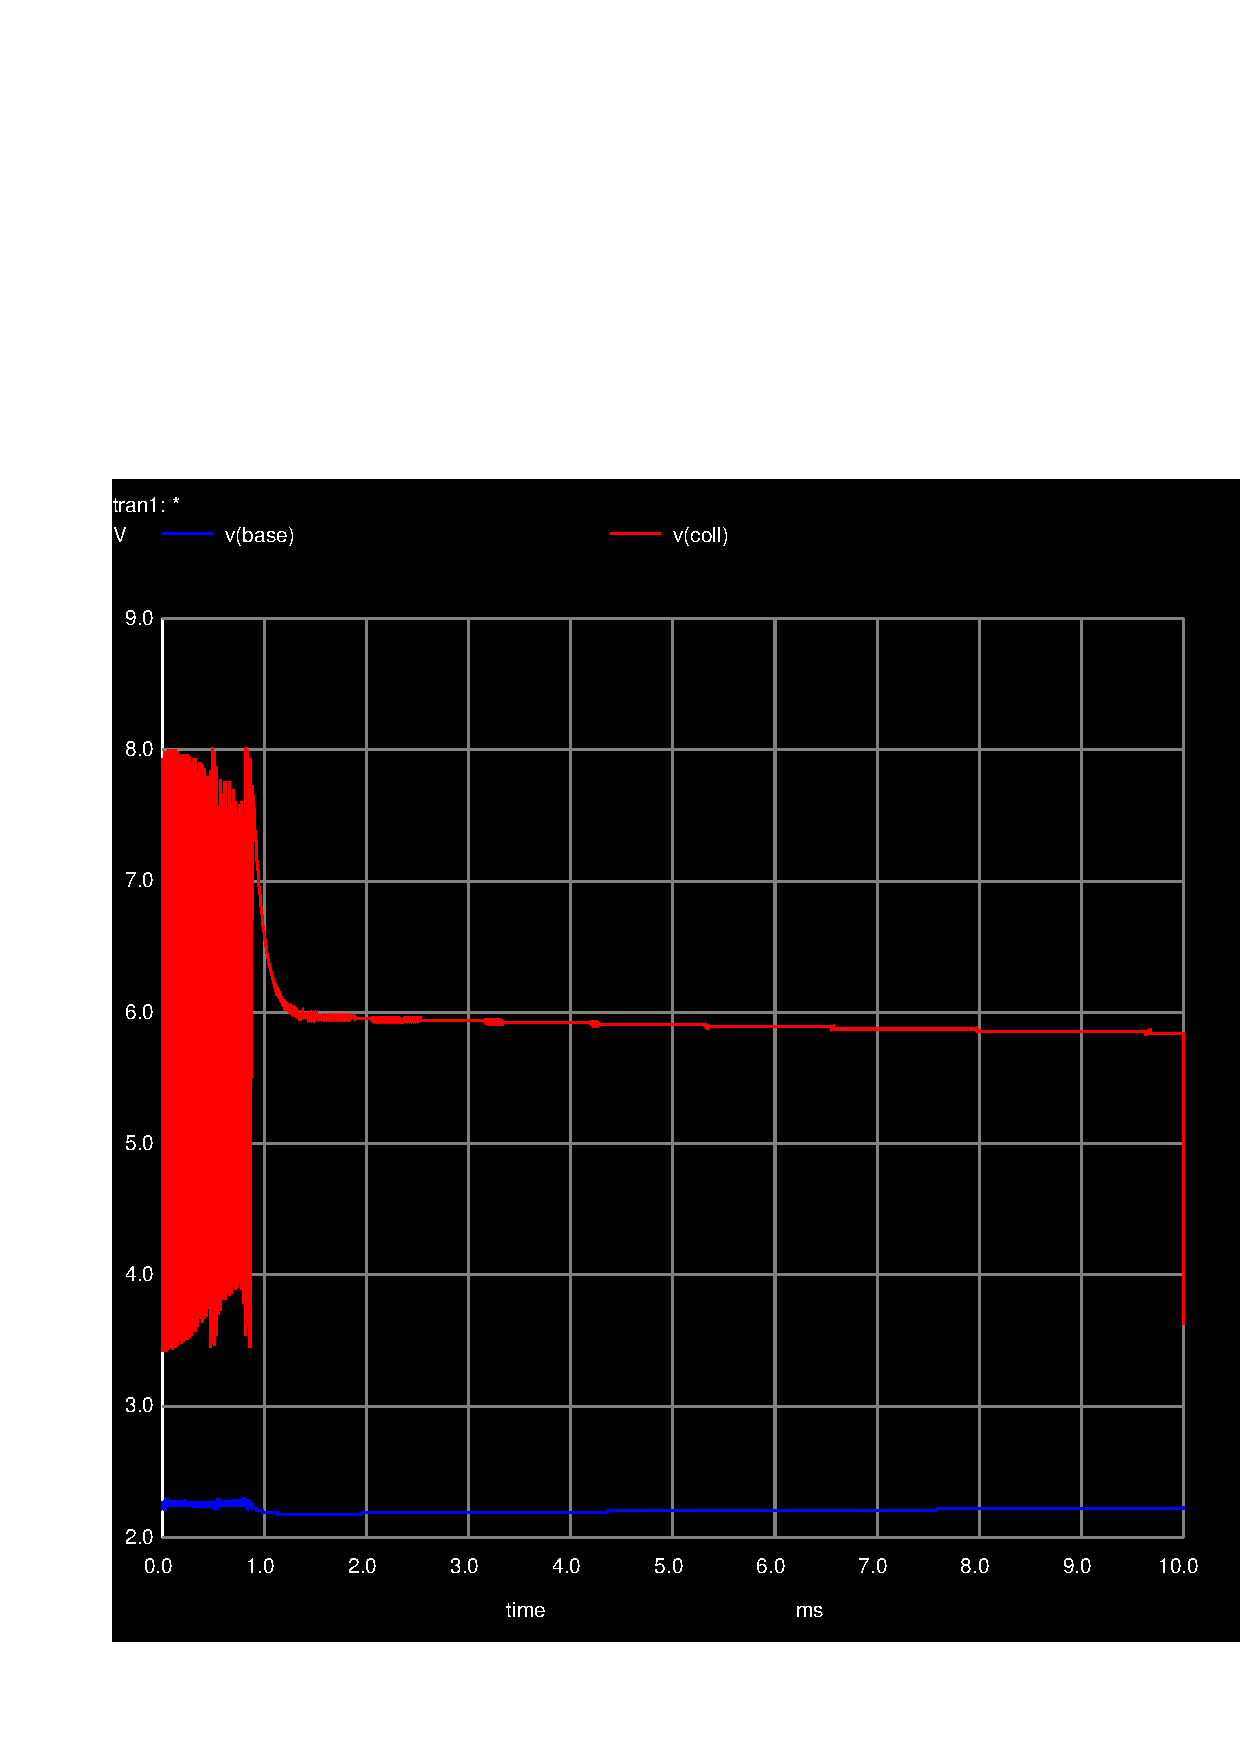
\includegraphics[width=0.6\linewidth]{trans.pdf}
\caption{Transient output voltage}
\label{fig:trans}
\end{figure}

\lipsum[1-1]



\subsection{Frequency Analysis}

\subsubsection{Magnitude Response}

Figure~\ref{fig:acm} shows the magnitude of the frequency response for the
circuit under analysis. Compared to the theoretical analysis results, one
notices the following differences: describe and explain the differences.

\begin{figure}[h] \centering
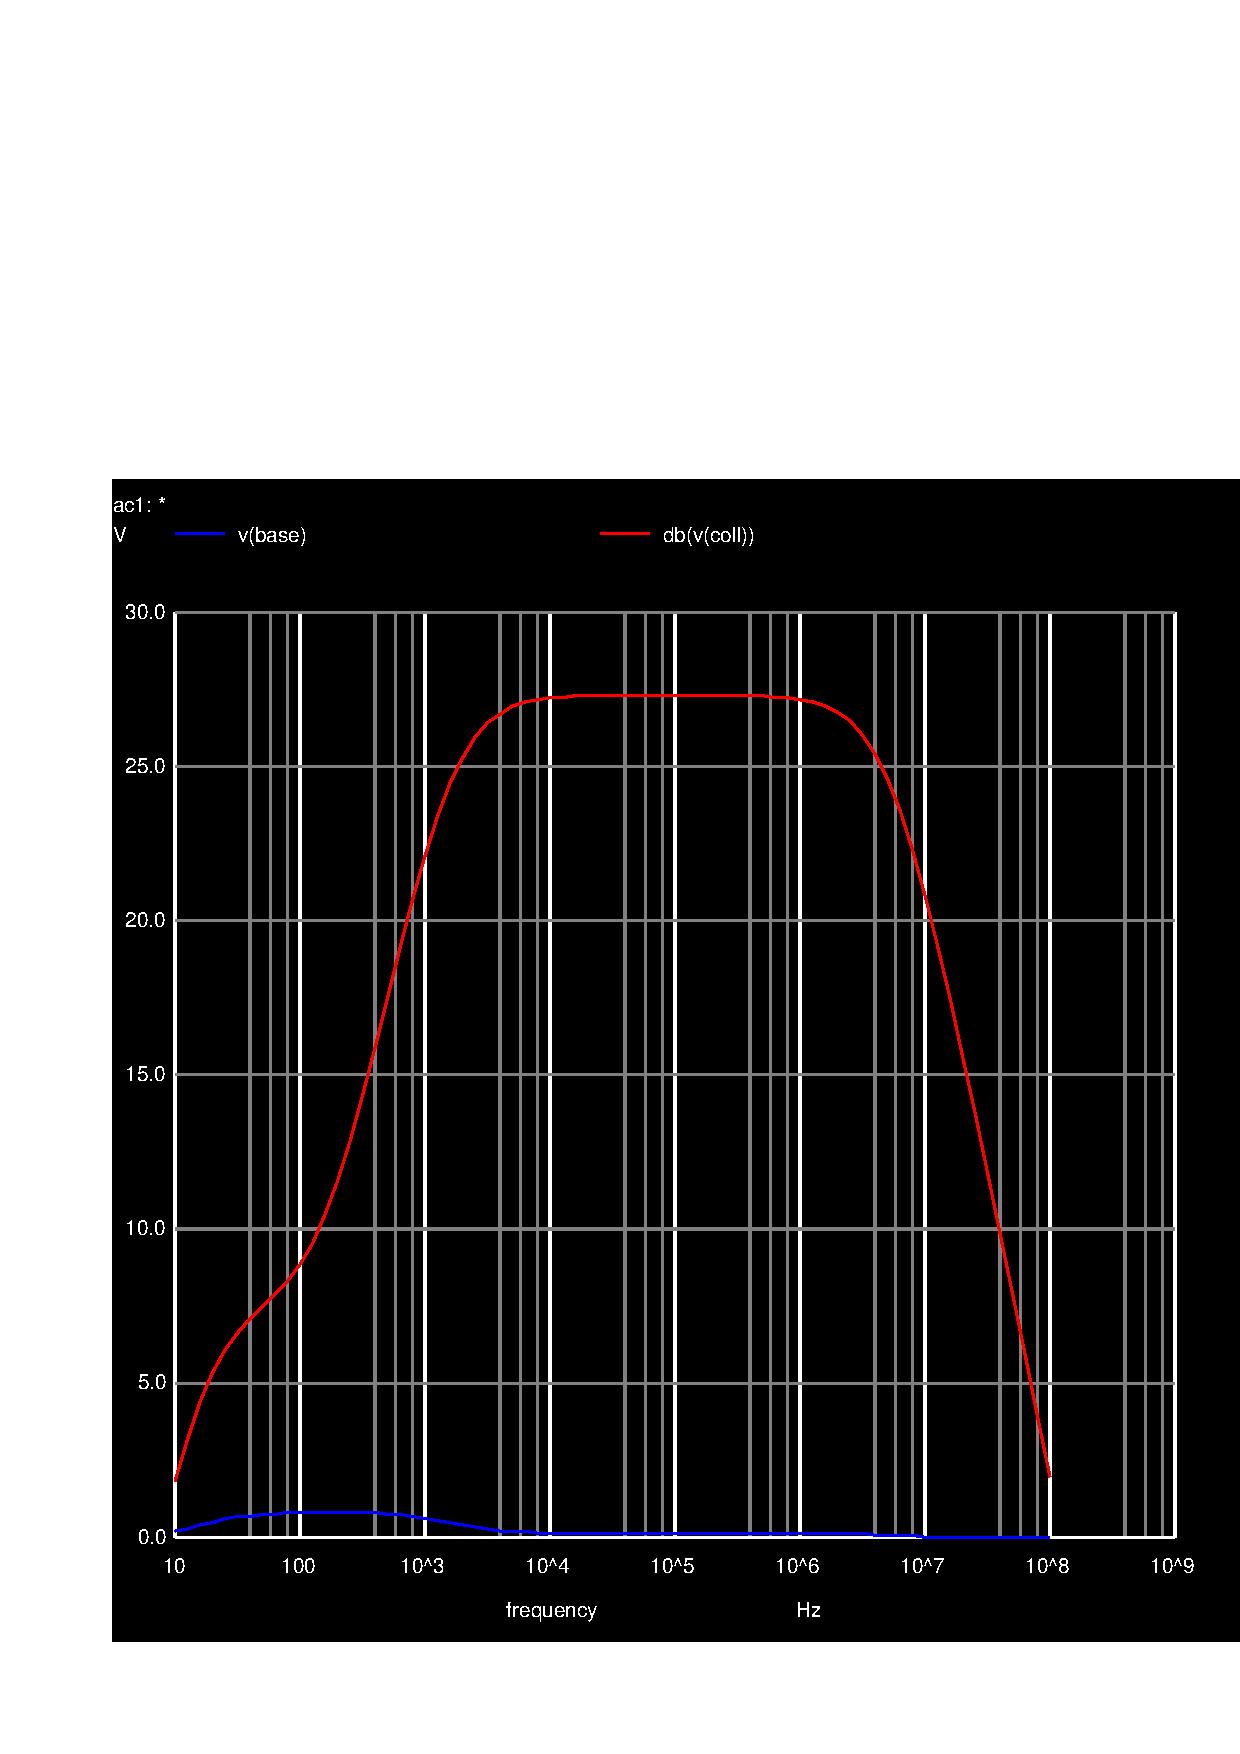
\includegraphics[width=0.6\linewidth]{acm.pdf}
\caption{Magnitude response}
\label{fig:acm}
\end{figure}

\lipsum[1-1]

\subsubsection{Phase Response}

Figure~\ref{fig:acp} shows the magnitude of the frequency response for the
circuit under analysis. Compared to the theoretical analysis results, one
notices the following differences: describe and explain the differences.

\begin{figure}[h] \centering
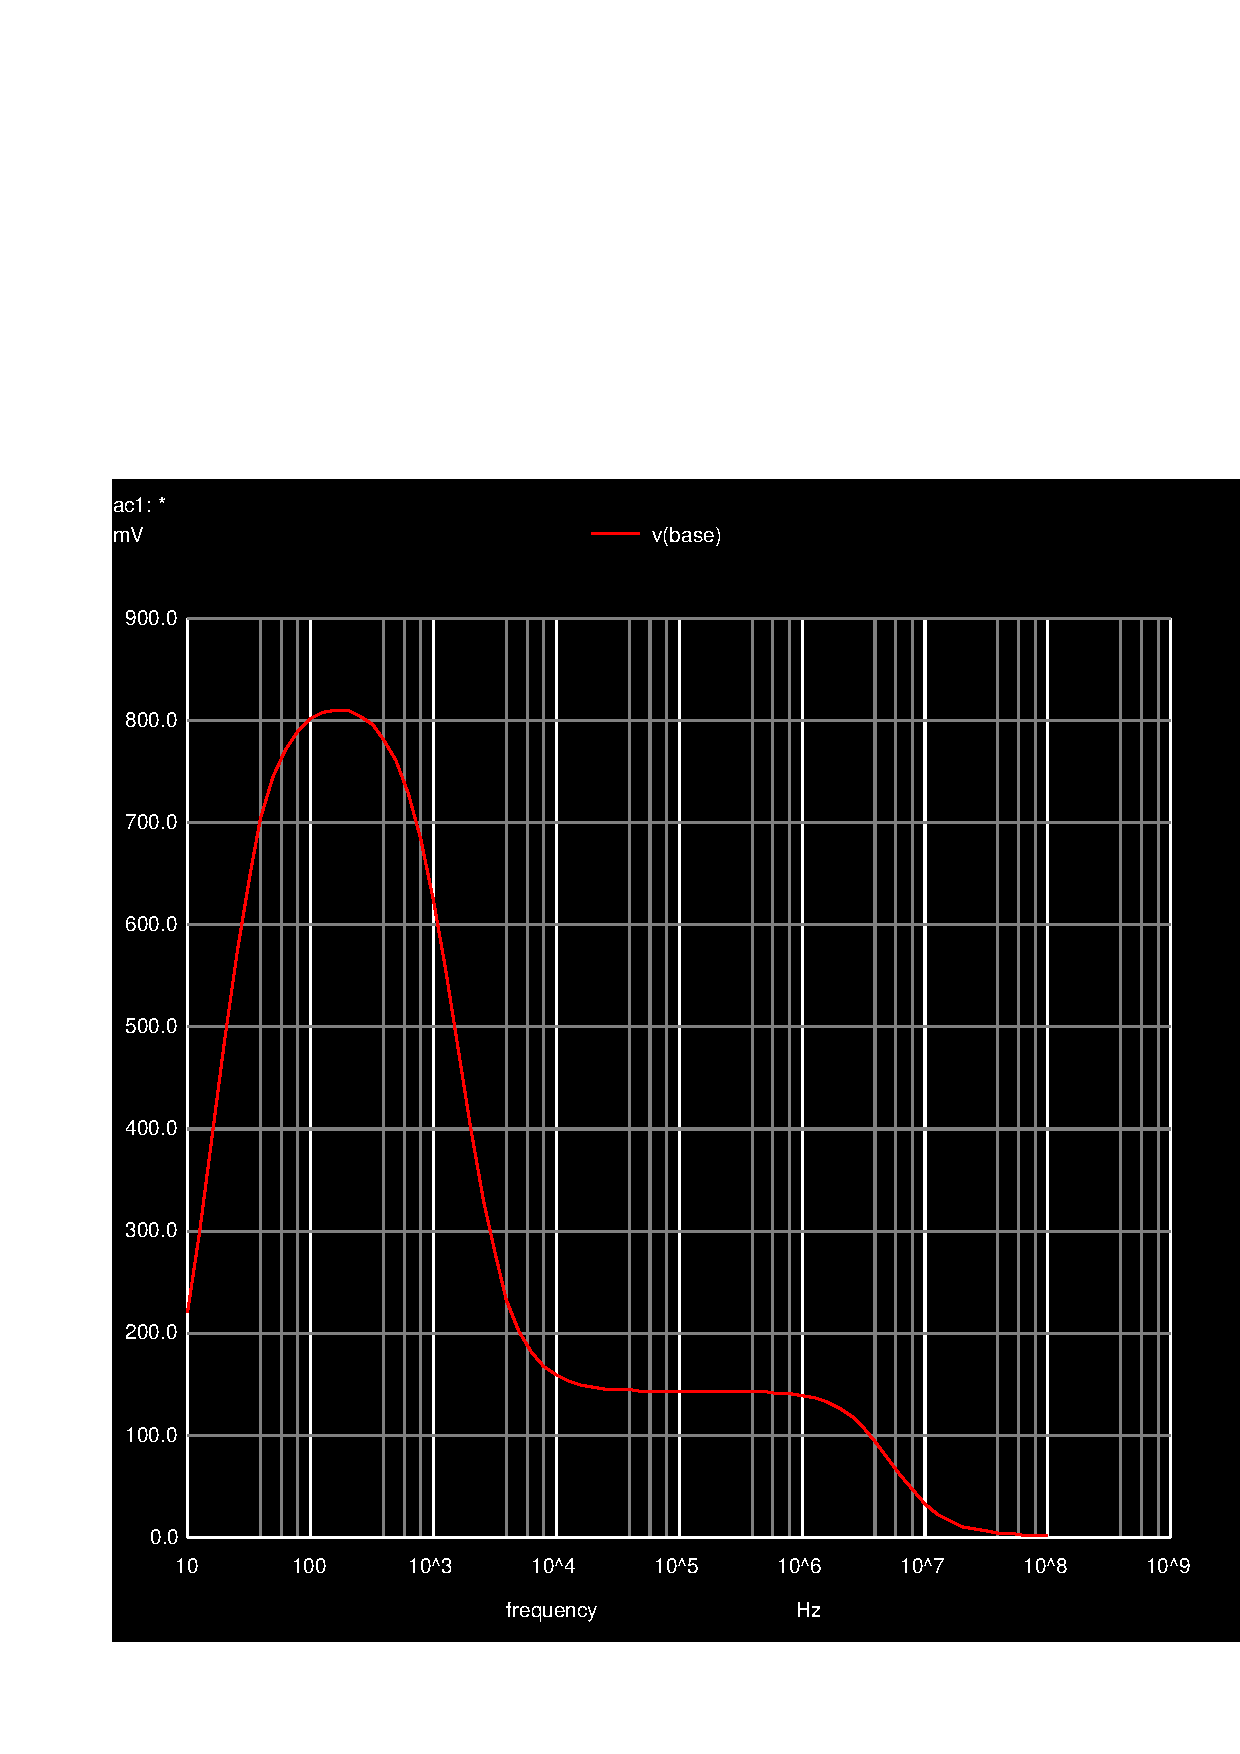
\includegraphics[width=0.6\linewidth]{acp.pdf}
\caption{Phase response}
\label{fig:acp}
\end{figure}

\lipsum[1-1]

\subsubsection{Input Impedance}

Figure~\ref{fig:zim} shows the magnitude of the frequency response for the
circuit under analysis. Compared to the theoretical analysis results, one
notices the following differences: describe and explain the differences.

\begin{figure}[h] \centering
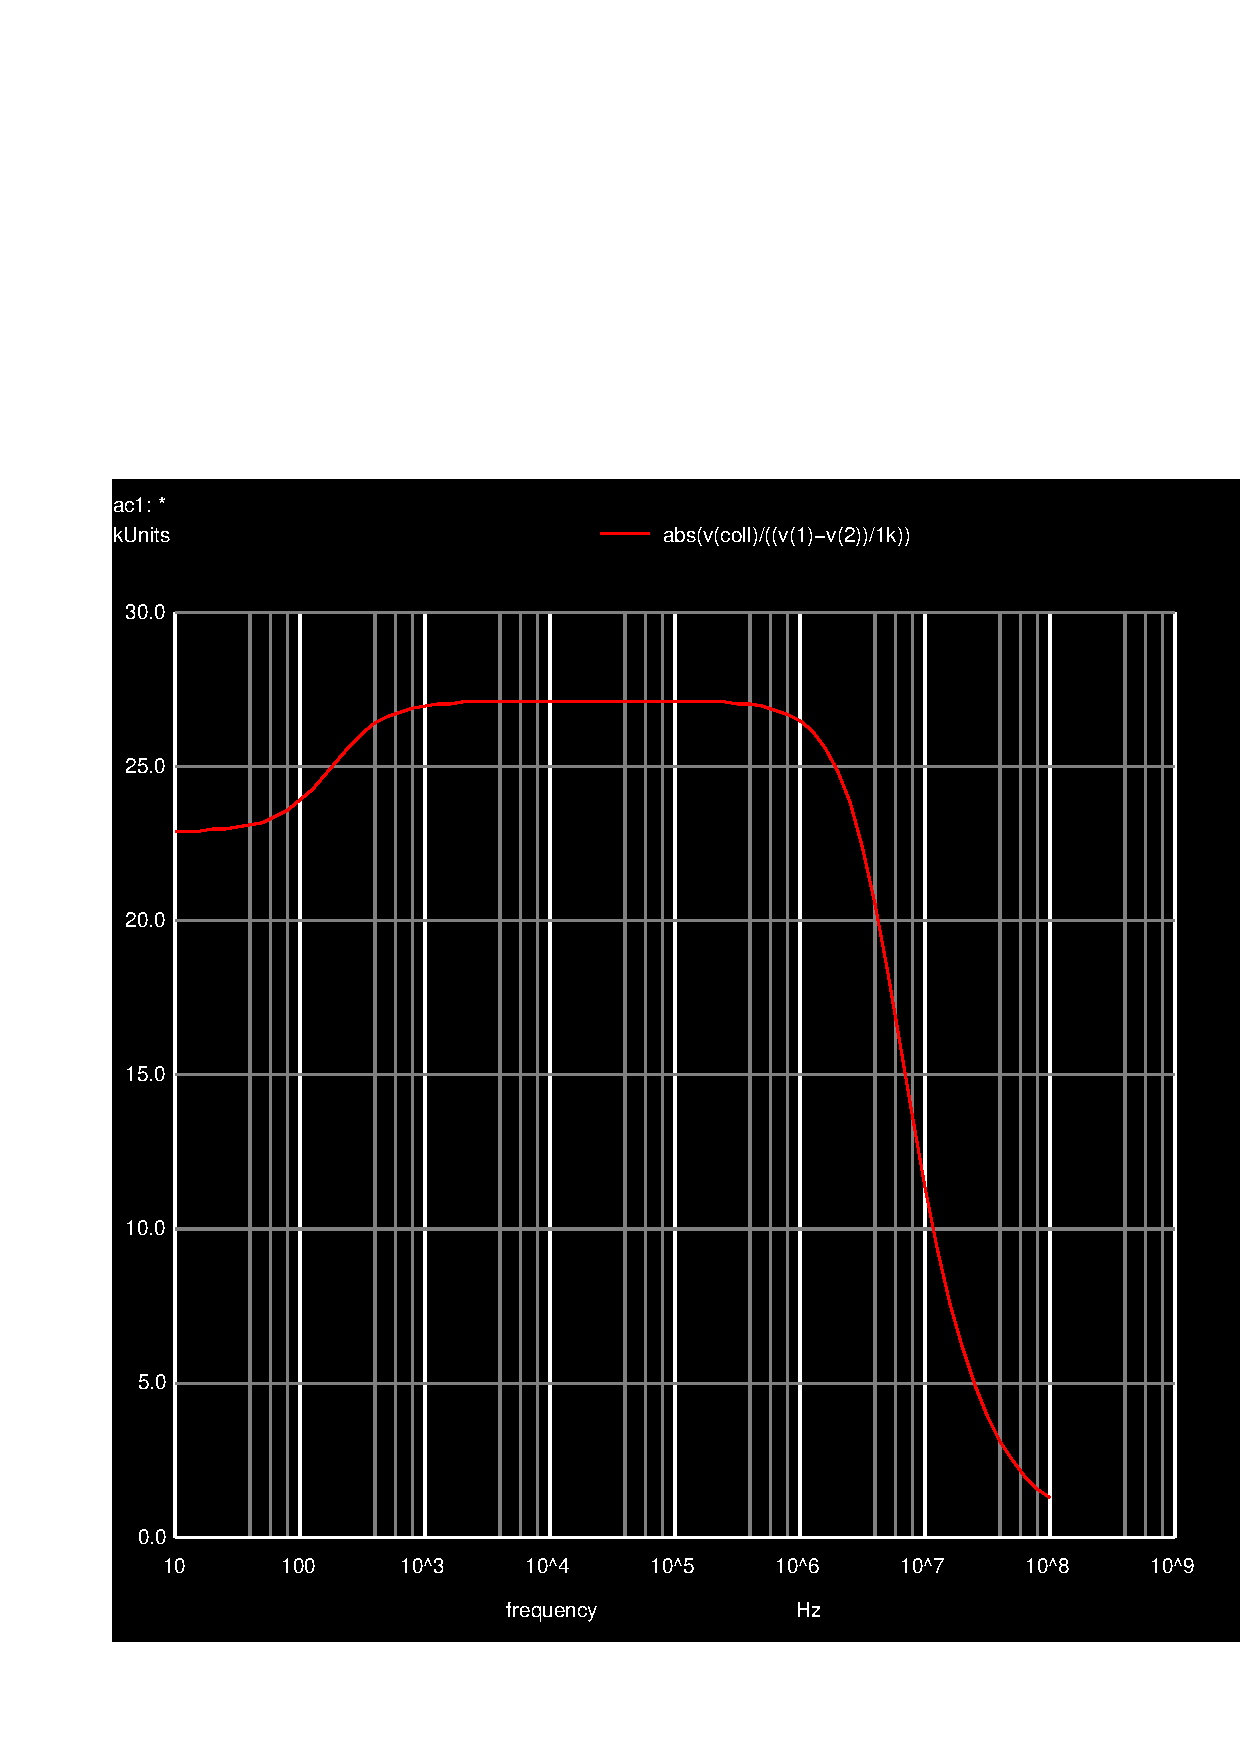
\includegraphics[width=0.6\linewidth]{zim.pdf}
\caption{Input impedance}
\label{fig:zim}
\end{figure}

\lipsum[1-1]



